% !TEX root = ../thesis.tex

\chapter{Meranie kvantových obvodov}

Jediným spôsobom ako zistiť skutočný stav kvnatového obvodu je meraním.
Merať možno všetky bity súčasne ako aj jednotlivé kvantové bity samostatne.

\section{Princíp merania kvantových obvodov}

Kvantový bit môže existovať v nekonečnom množstve stavov. Meranie si môžme 
predstaviť ako prevod stavov kvantových bitov do stavu klasického digitálneho
systému \cite{Nie10}. Pre príklad môžeme reprezentovať kvantový stav 
\(\alpha\ket{0} + \beta\ket{1}\) pomocou nulového a excitovaného stavu atómu.
Skutočný kvantový počítač by tak mohol merať tieto stavy. Pri meraní by 
daný atóm skolaboval do jedného zo stavov \(\ket{0}\) alebo \(\ket{1}\).
Pre kolabovanie samozrejme rovnako platí to, že do jednotlivých stavov by
sa atóm dostal s pravdepodobnosťami \(|\alpha|^2\) respektíve \(|\beta|^2\).


Pri každom fyzikálnom meraní nastáva určitá nepresnosť merania. Takisto 
pri meraní môže dokonca nastať zničenie obvodu. To vyplíva z toho, že pri
skolabovanom kvantovom bite nastáva zmena fizykálnych vlastností daného bitu. 

\section{Fiktívne meranie}

Našim cieľom je navrhnúť pravdepodobnostný model, ktorý by umožnil merať
stavy kvantových obvodov aj bez kolabovania jednotlivých kvantových bitov.

\subsection{Experiment 1}
Navrhnime kvantový obvod s dvoma bitmi. Označme ich \(\ket{\psi_0}\) a 
\(\ket{\psi_1}\). V prvom kroku aplikujeme Hadamardovo hrado na bit 
\(\ket{\psi_0}\). Nasledovať budú dve \(CNOT\) hradlá, s opačnými kontrólnymi 
a cieľovými bitmi. V IBM QX je tento obvod reprezenovaný ako 
\begin{code}
qreg q[2];
creg c[2];

h q[0];
cx q[0],q[1];
cx q[1],q[0];
\end{code}
Jeho grafické zobrazenie je na obrázku \ref{expr1_circuit}, aj s označenými
časovými úsekmi, v ktorých bude meraný stav systému. 

\begin{figure} 
	\centering 
	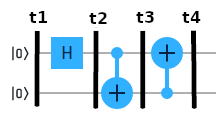
\includegraphics[width=.6\textwidth]{figures/expr1_circuit.png} 
	\caption{Jednotduchý kvantový obvod (namodelovaný v IBM Quantum Experience)}
    \label{expr1_circuit}
\end{figure}

\begin{itemize}
\item[] \textbf{Teoretická analýza} \\
Kvantové bity \(\ket{\psi_0}\) a \(\ket{\psi_2}\) sú definované ako 
\[\ket{\psi_0} = \alpha_0\ket{0} + \beta_0\ket{1}\]
\[\ket{\psi_1} = \alpha_1\ket{0} + \beta_1\ket{1}\]
, a teda je zrejmé, že v čase \(t_1\) pre celkový stav \(\ket{\psi}\) platí 
\[\ket{\psi} = \ket{\psi_0} \otimes \ket{\psi_1} = \alpha_0\alpha_1\ket{00} + \alpha_0\beta_1\ket{01} + \beta_0\alpha_1\ket{10} + \beta_0\beta_1\ket{11}\]

Z čoho jasne vyplíva, že systém nadobudne stav
    \begin{itemize}
        \item[] \(\ket{00}\) s pravdepodobnosťou \(|\alpha_0\alpha_1 |^2\)
        \item[] \(\ket{01}\) s pravdepodobnosťou \(| \alpha_0\beta_1 |^2\)
        \item[] \(\ket{10}\) s pravdepodobnosťou \(| \beta_0\alpha_1 |^2\)
        \item[] \(\ket{11}\) s pravdepodobnosťou \(| \beta_0\beta_1 |^2\) 
    \end{itemize}

Po prechode Hadamardovim hradlom, v čase \(t_2\) kvantové bity zmenia stav na
\[\ket{\psi_0} = \frac{\alpha_0 + \beta_0}{\sqrt{2}}\ket{0} + \frac{\alpha_0 - \beta_0}{\sqrt{2}}\ket{1}\]
\[\ket{\psi_1} = \alpha_1\ket{0} + \beta_1\ket{1}\]

, a teda pre celkový stav \(\ket{\psi}\) bude platiť
\[\ket{\psi} = \frac{\alpha_0 + \beta_0}{\sqrt{2}}\alpha_1\ket{00} + \frac{\alpha_0 + \beta_0}{\sqrt{2}}\beta_1\ket{01} + \frac{\alpha_0 - \beta_0}{\sqrt{2}}\alpha_1\ket{10} + \frac{\alpha_0 - \beta_0}{\sqrt{2}}\beta_1\ket{11}\]

Kvantoý systém kolabuje do stavu
    \begin{itemize}
        \item[] \(\ket{00}\) s pravdepodobnosťou \(|\frac{\alpha_0 + \beta_0}{\sqrt{2}}\alpha_1|^2\)
        \item[] \(\ket{01}\) s pravdepodobnosťou \(|\frac{\alpha_0 + \beta_0}{\sqrt{2}}\beta_1|^2\)
        \item[] \(\ket{10}\) s pravdepodobnosťou \(|\frac{\alpha_0 - \beta_0}{\sqrt{2}}\alpha_1|^2\)
        \item[] \(\ket{11}\) s pravdepodobnosťou \(|\frac{\alpha_0 - \beta_0}{\sqrt{2}}\beta_1|^2\) 
    \end{itemize}

\end{itemize}

\subsection{Experiment 2}
\subsection{Experiment 3}
